% !TeX root = ../../Book1.tex
% 纲要标题：### 11.3 局部逆与秩定理
% 纲要位置：几何学计划纲要.md，第 551 行。
% 正文状态：初稿；尚未正式审核。

% 纲要内容开始
% 
% * 逆函数定理的定量局部证明
% * 隐函数定理与参数依赖
% * 常秩定理的坐标约化
% * 秩不恒定时的反例
% 
% 纲要内容结束

\section{局部逆与秩定理}
\label{g1:sec:1103}

微分把光滑映射在一点附近的变化近似为线性映射。如果这个线性映射可逆，原映射是否也能在附近反解？如果微分只保留一部分方向，能否用坐标把这部分方向同被压缩的方向分开？这两个问题分别由逆函数定理与常秩定理回答。本节从有限维微积分和线性代数重新证明所需结论，具体说明邻域如何选择、反解为何光滑，以及秩的条件用在什么地方。

\subsection{逆函数定理的定量局部证明}
\label{g1:subsec:1103:01}

先把问题放在 \(\mathbb R^n\) 中。Euclid 范数记为 \(|\cdot|\)，矩阵使用对应的算子范数 \(\|A\|=\sup_{|v|=1}|Av|\)。记 \(B_r(a)\) 为开球，\(\overline B_r(a)\) 为闭球；省略中心时指中心为零。对 Euclid 映射写 \(\mathrm{D}f(x)\) 表示导数矩阵，它表示上一节中微分 \(\mathrm{d}f_x\) 在标准坐标基下的矩阵，并不是一种新的求导运算。

\ProseParagraphBreak

如果已经通过平移与可逆线性变换化成 \(f(0)=0\)、\(\mathrm{D}f(0)=I\)，那么 \(f(x)\) 在原点附近接近 \(x\)。将 \(f(x)=y\) 改写为
\[
	x=y-\bigl(f(x)-x\bigr)
\]
就给出一个逐步修正的办法：先猜一个 \(x\)，再减去它偏离目标的误差。我们需要的不是这一步误差必然很小，而是两次猜测经过修正后彼此更接近。下面的引理把这个思路变成收敛证明。

\begin{lemma}[压缩映射]
	\label{g1:lem:euclidean-contraction}
	设 \(K=\overline B_r(a)\subset\mathbb R^n\) 是非空闭球，\(T:K\to K\) 满足
	\[
		|T(x)-T(x')|\leq q|x-x'|,\qquad 0\leq q<1.
	\]
	则 \(T\) 有唯一不动点 \(x_*\)。从任意 \(x_0\in K\) 出发，递推 \(x_{j+1}=T(x_j)\)，均收敛到 \(x_*\)；当 \(0<q<1\) 时有
	\[
		|x_j-x_*|\leq\frac{q^j}{1-q}|x_1-x_0|.
	\]
\end{lemma}
\begin{proof}
	若 \(q=0\)，映射 \(T\) 为常值，第二次迭代起就不再变化，结论立即成立。以下设 \(0<q<1\)。由归纳，
	\[
		|x_{j+1}-x_j|\leq q^j|x_1-x_0|.
	\]
	对 \(k>j\)，三角不等式和几何级数给出
	\[
		|x_k-x_j|\leq\sum_{\ell=j}^{k-1}|x_{\ell+1}-x_\ell|
		\leq\frac{q^j}{1-q}|x_1-x_0|.
	\]
	因此各坐标都是实数 Cauchy 序列，逐坐标收敛给出 \(\mathbb R^n\) 中的极限 \(x_*\)。闭球的闭性保证 \(x_*\in K\)，而压缩不等式蕴含 \(T\) 连续，所以取极限得 \(x_*=T(x_*)\)。让上式中的 \(k\to\infty\)，也得到误差估计。若还有不动点 \(z_*\)，则
	\[
		|x_*-z_*|=|T(x_*)-T(z_*)|\leq q|x_*-z_*|,
	\]
	因 \(q<1\)，只能有 \(x_*=z_*\)。
\end{proof}

闭球在这里承担两个不同职责：迭代不能跑出定义域，极限也不能掉到定义域之外。严格不等式 \(q<1\) 则使累计误差成为收敛的几何级数。仅有“距离不增加”不能给出同一结论，例如闭球上的恒等映射有许多不动点。

\begin{theorem}[定量局部逆]
	\label{g1:thm:quantitative-inverse-function}
	设 \(n\geq1\)，\(f:U\to\mathbb R^n\) 为 \(C^k\) 映射，其中 \(U\subset\mathbb R^n\) 开，\(1\leq k\leq\infty\)。假设 \(\overline B_r\subset U\)、\(r>0\)，且
	\[
		f(0)=0,\qquad \mathrm{D}f(0)=I,\qquad
		\sup_{x\in\overline B_r}\|\mathrm{D}f(x)-I\|\leq q<1,\quad q\geq0.
	\]
	则 \(f\) 在 \(\overline B_r\) 上单射，且对 \(x,x'\in\overline B_r\)，
	\begin{equation}
		\label{g1:eq:quantitative-inverse-bounds}
		(1-q)|x-x'|\leq|f(x)-f(x')|\leq(1+q)|x-x'|.
	\end{equation}
	像 \(\Omega=f(B_r)\) 是开集，并满足
	\[
		B_{(1-q)r}\subset\Omega.
	\]
	映射 \(f:B_r\to\Omega\) 是 \(C^k\) 微分同胚。其逆映射 \(g\) 满足
	\begin{equation}
		\label{g1:eq:inverse-derivative}
		\mathrm{D}g(y)=\bigl(\mathrm{D}f(g(y))\bigr)^{-1},\qquad
		|g(y)-g(y')|\leq\frac{|y-y'|}{1-q}.
	\end{equation}
	特别地，对 \(|y|<(1-q)r\)，方程 \(f(x)=y\) 在 \(B_r\) 内有唯一解，而且 \(|x|\leq|y|/(1-q)\)。
\end{theorem}
\begin{proof}
	令 \(E(x)=f(x)-x\)。闭球是凸的，所以任意两点间的线段仍在闭球中。对函数 \(t\mapsto E(x'+t(x-x'))\) 逐分量应用一元微积分基本定理，得到
	\[
		E(x)-E(x')=\int_0^1\mathrm{D}E(x'+t(x-x'))(x-x')\,\mathrm{d}t.
	\]
	因此 \(|E(x)-E(x')|\leq q|x-x'|\)。在 \(f(x)-f(x')=(x-x')+(E(x)-E(x'))\) 中分别使用三角不等式及其反向形式，便得\eqref{g1:eq:quantitative-inverse-bounds}，特别地 \(f\) 单射。

	固定 \(|y|\leq(1-q)r\)，令 \(T_y(x)=y-E(x)\)。因为 \(E(0)=0\)，对 \(x\in\overline B_r\) 有
	\[
		|T_y(x)|\leq|y|+q|x|\leq r.
	\]
	所以它把闭球映入自身，且压缩因子至多为 \(q\)。\cref{g1:lem:euclidean-contraction}给出唯一不动点 \(x\)，不动点方程正是 \(f(x)=y\)。再由\eqref{g1:eq:quantitative-inverse-bounds}取 \(x'=0\)，得到 \(|x|\leq|y|/(1-q)\)。当目标满足严格不等式时，解在开球内，从而证明 \(B_{(1-q)r}\subset f(B_r)\)。

	还须证明整个像 \(\Omega\) 开，而不能只知道它包含原点附近的一个球。任取 \(x_0\in B_r\)，选 \(\rho>0\) 使 \(\overline B_\rho(x_0)\subset B_r\)。对
	\[
		|y-f(x_0)|<(1-q)\rho
	\]
	仍使用同一个 \(T_y\)。此时
	\[
		|T_y(x)-x_0|
		\leq|y-f(x_0)|+|E(x)-E(x_0)|
		\leq|y-f(x_0)|+q\rho<\rho.
	\]
	它把这个较小闭球映入自身，故每个这样的 \(y\) 都在 \(f(B_r)\) 中。这就证明了 \(\Omega\) 开。\eqref{g1:eq:quantitative-inverse-bounds}又立即给出逆映射的 Lipschitz 估计，所以 \(g\) 首先是连续的。

	对任意 \(x\in B_r\) 与向量 \(v\)，导数条件给出 \(|\mathrm{D}f(x)v|\geq(1-q)|v|\)。故 \(\mathrm{D}f(x)\) 单射；由于定义域和值域维数同为 \(n\)，它可逆，并且 \(\|\mathrm{D}f(x)^{-1}\|\leq(1-q)^{-1}\)。固定 \(y=f(x)\)，对充分小的 \(h\) 令 \(\xi=g(y+h)-x\)。逆映射的 Lipschitz 估计给出 \(|\xi|\leq|h|/(1-q)\)。利用 \(f\) 在 \(x\) 的可微性，
	\[
		h=\mathrm{D}f(x)\xi+o(|\xi|),
		\qquad
		\xi=\mathrm{D}f(x)^{-1}h+o(|h|).
	\]
	这正是 \(g\) 在 \(y\) 可微及\eqref{g1:eq:inverse-derivative}的含义。

	矩阵求逆在可逆矩阵集合上光滑：每个矩阵元由伴随矩阵的多项式除以非零行列式给出。因 \(\mathrm{D}f\) 与 \(g\) 连续，导数公式先使 \(\mathrm{D}g\) 连续，故 \(g\in C^1\)。若 \(f\in C^k\)，且已经知道 \(g\in C^j\)、\(j<k\)，则 \(\mathrm{D}f\in C^{k-1}\)，同一公式使 \(\mathrm{D}g\in C^j\)，于是 \(g\in C^{j+1}\)。逐阶归纳得到 \(C^k\)；当 \(k=\infty\) 时，对每个有限阶作此归纳即可。
\end{proof}

这里的定量信息不仅是逆映射存在。\((1-q)r\) 给出一个必定包含在像中的目标半径，\((1-q)^{-1}\) 控制反解对目标误差的放大。实际像可以更大；定理只承诺由当前导数界能够保证的部分。

\begin{theorem}[逆函数定理]
	\label{g1:thm:inverse-function}
	设 \(f:U\subset\mathbb R^n\to\mathbb R^n\) 为 \(C^k\) 映射，\(U\) 开，\(1\leq k\leq\infty\)。若 \(\mathrm{D}f(a)\) 可逆，则存在 \(a\) 与 \(f(a)\) 的开邻域 \(U_0,V_0\)，使 \(f:U_0\to V_0\) 为 \(C^k\) 微分同胚。
	
	相应地，若 \(M,N\) 是同维无边界光滑流形，\(F:M\to N\) 光滑，且 \(\mathrm{d}F_p:\mathrm{T}_pM\to \mathrm{T}_{F(p)}N\) 为线性同构，则 \(F\) 在 \(p\) 的某个开邻域上为到 \(F(p)\) 开邻域的微分同胚。
\end{theorem}
\begin{proof}
	设 \(A=\mathrm{D}f(a)\)。对 \(h\) 接近零，定义
	\[
		\widetilde f(h)=A^{-1}\bigl(f(a+h)-f(a)\bigr).
	\]
	则 \(\widetilde f(0)=0\)、\(\mathrm{D}\widetilde f(0)=I\)。导数的连续性允许选取 \(r>0\) 及 \(q<1\)，例如 \(q=1/2\)，使闭球包含在定义域中，且 \(\|A^{-1}\mathrm{D}f(a+h)-I\|\leq q\) 在闭球上成立。应用\cref{g1:thm:quantitative-inverse-function}，再还原平移与线性变换，便得第一部分。

	流形情形，在 \(p\) 与 \(F(p)\) 附近选坐标图。\cref{g1:prop:differential-chain-rule}说明，坐标表达的微分是在 \(\mathrm{d}F_p\) 两侧复合坐标微分同构，故也是可逆矩阵。将 Euclid 结论应用于这一坐标表达，再用坐标图送回流形，得到所需邻域及光滑逆。零维情形的坐标域是单点，结论直接成立。
\end{proof}

一般情形仍有明确尺度。若归一化后的导数界在 \(\overline B_r(a)\) 上为 \(q\)，则
\[
	f(a)+A B_{(1-q)r}\subset f(B_r(a)).
\]
特别地，像包含以 \(f(a)\) 为中心、半径 \((1-q)r/\|A^{-1}\|\) 的 Euclid 球；在这个像上的逆映射满足 Lipschitz 常数不超过 \(\|A^{-1}\|/(1-q)\)。这里先乘 \(A^{-1}\) 的作用，是把原映射在该点不同方向的线性伸缩统一成恒等变换。

\begin{example}
	\label{g1:exm:local-global-inverse}
	映射 \(f(s,t)=(e^s\cos t,e^s\sin t)\) 的导数行列式为 \(e^{2s}>0\)，因此在每一点附近都可光滑反解。但 \(f(s,t+2\pi)=f(s,t)\)，故它不是全局单射。逆函数定理确定的是一个足够小的邻域，并没有把不同邻域的逆自动拼成全局逆。
\end{example}

\subsection{隐函数定理与参数依赖}
\label{g1:subsec:1103:02}

方程 \(F(x,y)=0\) 往往已经给出一个几何对象，却没有把它写成函数图像。若 \(y\) 方向的变化能独立控制全部方程，就有希望把 \(y\) 解成 \(x\) 的函数。为把这个问题转成逆函数问题，保留 \(x\) 不动，把新的另一组坐标取为方程值 \(F\)；然后令这组新坐标等于零。

\begin{theorem}[带参数的隐函数定理]
	\label{g1:thm:implicit-function-parameters}
	设 \(\Omega\subset\mathbb R^p\times\mathbb R^n\times\mathbb R^m\) 开，\(m\geq1\)，\(p,n\geq0\)，且 \(F:\Omega\to\mathbb R^m\) 为 \(C^k\) 映射，\(1\leq k\leq\infty\)。将变量写成 \((\lambda,x,y)\)，并假设
	\[
		F(\lambda_0,x_0,y_0)=0,\qquad \mathrm{D}_yF(\lambda_0,x_0,y_0)\ \text{可逆}.
	\]
	则存在三个点各自的开邻域 \(P,U,V\)，使 \(P\times U\times V\subset\Omega\)，并存在唯一 \(C^k\) 映射 \(\varphi:P\times U\to V\)，满足
	\begin{equation}
		\label{g1:eq:implicit-graph}
		F(\lambda,x,y)=0
		\quad\Longleftrightarrow\quad
		y=\varphi(\lambda,x)
		\qquad((\lambda,x,y)\in P\times U\times V).
	\end{equation}
	缩小这些邻域后，\(\mathrm{D}_yF\) 在其中可逆，而且
	\begin{equation}
		\label{g1:eq:implicit-derivative}
		\mathrm{D}_{(\lambda,x)}\varphi
		=-\bigl(\mathrm{D}_yF(\lambda,x,\varphi)\bigr)^{-1}
		\mathrm{D}_{(\lambda,x)}F(\lambda,x,\varphi).
	\end{equation}
\end{theorem}
\begin{proof}
	合并记 \(z=(\lambda,x)\)，并构造
	\[
		H(z,y)=(z,F(z,y)).
	\]
	其在基点的导数矩阵为
	\[
		\mathrm{D}H=\begin{pmatrix}I&0\\\mathrm{D}_zF&\mathrm{D}_yF\end{pmatrix}.
	\]
	这个矩阵可逆：若给定输出增量 \((a,b)\)，先取输入的 \(z\) 增量为 \(a\)，再取 \(y\) 增量为 \((\mathrm{D}_yF)^{-1}(b-\mathrm{D}_zF\,a)\)，就得到唯一解。由\cref{g1:thm:inverse-function}，\(H\) 在基点附近是微分同胚。因为第一组坐标始终保持为 \(z\)，它的逆必写成
	\[
		H^{-1}(z,w)=(z,\psi(z,w)).
	\]
	令 \(\varphi(z)=\psi(z,0)\)，便得到光滑候选解。

	需要确保存在性与唯一性在同一个乘积邻域上成立。先在 \(H\) 的可逆邻域内取基点的一个小乘积盒 \(Z_1\times V\)。目标可逆邻域是开集，因此缩小 \(Z_1\) 后，所有 \((z,0)\) 都落在目标可逆邻域中；再由 \(\psi(z_0,0)=y_0\) 及连续性，进一步缩小 \(Z_1\)，使 \(\psi(z,0)\in V\)。最后在这组 \(z\) 邻域中取乘积 \(P\times U\)。于是每个 \((\lambda,x)\in P\times U\) 都有解 \(\varphi(\lambda,x)\in V\)；任何另一个 \(y\in V\) 若使 \(F=0\)，就与该解经 \(H\) 具有同一像 \((\lambda,x,0)\)，由 \(H\) 在所取邻域中的单射性，二者相等。这证明\eqref{g1:eq:implicit-graph}。

	行列式连续且基点处非零，故还可把乘积邻域缩小到 \(\mathrm{D}_yF\) 始终可逆。对恒等式 \(F(\lambda,x,\varphi(\lambda,x))=0\) 使用链式法则，得到
	\[
		\mathrm{D}_{(\lambda,x)}F+\mathrm{D}_yF\,\mathrm{D}_{(\lambda,x)}\varphi=0,
	\]
	左乘 \((\mathrm{D}_yF)^{-1}\) 便得导数公式。
\end{proof}

参数 \(\lambda\) 在证明中也是变量。把它并入 \(z\)，使我们一次得到对参数与自变量的联合光滑性，而不只知道“每个固定参数分别有一个解”。唯一性也有明确范围：它只排除所选 \(V\) 内的第二个解，不排除其他地方还有另一条分支。

\begin{example}
	\label{g1:exm:parameter-circle-implicit}
	令 \(F(\lambda,x,y)=x^2+y^2-\lambda\)。在 \((\lambda,x,y)=(1,0,1)\) 处有 \(\mathrm{D}_yF=2\)，所以在附近存在唯一接近 \(1\) 的解
	\[
		y=\varphi(\lambda,x)=\sqrt{\lambda-x^2}.
	\]
	导数公式给出 \(\partial_\lambda\varphi=1/(2\varphi)\)、\(\partial_x\varphi=-x/\varphi\)，与直接求导一致。附近另有接近 \(-1\) 的解，但它不在当前的 \(V\) 中。到了 \(\lambda=x^2\) 且 \(y=0\) 时，\(\mathrm{D}_yF=0\)，这条光滑反解不能照原坐标方式继续；当 \(\lambda<x^2\) 时更没有实数解。对参数的局部光滑依赖并不承诺参数任意变化后仍有同一条光滑分支。
\end{example}

隐函数定理也没有指定哪些字母天生是未知量。若另一组 \(m\) 个变量对应的偏导数块可逆，就可以把它们作为待解变量；余下变量成为自变量或参数。选择可逆子块的办法，正是常秩定理的起点。

\subsection{常秩定理的坐标约化}
\label{g1:subsec:1103:03}

现在允许源空间与目标空间维数不同。一个秩为 \(r\) 的线性映射，经过两边换基可写成 \((u_1,\ldots,u_m)\mapsto(u_1,\ldots,u_r,0,\ldots,0)\)。非线性映射未必等于其线性近似，但如果微分的秩在附近始终为 \(r\)，就能用光滑坐标变化得到同样的局部形式。证明会先把 \(r\) 个输出直接用作源坐标，再说明其余输出不再含新的独立变化。

\begin{theorem}[常秩定理]
	\label{g1:thm:constant-rank}
	设 \(f:U\subset\mathbb R^m\to\mathbb R^n\) 为光滑映射，\(U\) 开，且 \(\operatorname{rank}\mathrm{D}f(x)=r\) 在 \(a\) 的某个邻域内恒成立，其中 \(0\leq r\leq\min(m,n)\)。则存在 \(a\) 的开邻域 \(U_0\)、\(f(a)\) 的开邻域 \(V_0\)，以及光滑坐标变换
	\[
		\phi:U_0\longrightarrow\widetilde U,\qquad
		\psi:V_0\longrightarrow\widetilde V,
	\]
	使 \(f(U_0)\subset V_0\)、\(\phi(a)=0\)、\(\psi(f(a))=0\)，并且
	\begin{equation}
		\label{g1:eq:constant-rank-normal-form}
		(\psi\circ f\circ\phi^{-1})(u_1,\ldots,u_m)
		=(u_1,\ldots,u_r,0,\ldots,0).
	\end{equation}
	最后一组零共有 \(n-r\) 个。
\end{theorem}
\begin{proof}
	先设 \(r>0\)。平移源与目标，使 \(a=0\)、\(f(a)=0\)。秩为 \(r\) 意味着 \(\mathrm{D}f(0)\) 有一个 \(r\) 阶子式非零；重排源、目标坐标后，可设左上角的 \(r\times r\) 子块可逆。记 \(x=(x',x'')\)，其中 \(x'\in\mathbb R^r\)、\(x''\in\mathbb R^{m-r}\)，并定义
	\[
		H(x)=\bigl(f_1(x),\ldots,f_r(x),x''\bigr).
	\]
	它的导数为分块上三角矩阵，左上角正是所选可逆块，右下角是 \(I_{m-r}\)，故 \(\mathrm{D}H(0)\) 可逆。逆函数定理给出 \(H\) 的局部光滑逆。把新源坐标记为 \((u,v)=H(x)\)，则
	\[
		(f\circ H^{-1})(u,v)=(u,G(u,v)).
	\]
	这一步的含义是把已经知道彼此独立的 \(r\) 个输出变成前 \(r\) 个输入坐标。

	链式法则以及 \(\mathrm{D}H^{-1}\) 可逆，保证改换源坐标后秩仍为 \(r\)。另一方面，
	\[
		\mathrm{D}(f\circ H^{-1})
		=\begin{pmatrix}I_r&0\\\mathrm{D}_uG&\mathrm{D}_vG\end{pmatrix}.
	\]
	从下方各行减去 \(\mathrm{D}_uG\) 给出的前 \(r\) 行线性组合，得到 \(\begin{psmallmatrix}I_r&0\\0&\mathrm{D}_vG\end{psmallmatrix}\)，其秩是 \(r+\operatorname{rank}\mathrm{D}_vG\)。因此常秩假设迫使 \(\mathrm{D}_vG=0\) 在整个所取邻域内成立；只知道基点处的秩为 \(r\)，无法得到这一步。

	缩小到以零为中心的乘积球 \(B'\times B''\)，使整个乘积都位于新坐标域中。对固定 \(u\)，线段 \(t\mapsto tv\) 始终在 \(B''\) 中，故微积分基本定理给出
	\[
		G(u,v)-G(u,0)=\int_0^1\mathrm{D}_vG(u,tv)v\,\mathrm{d}t=0.
	\]
	令 \(g(u)=G(u,0)\)，于是 \(f\circ H^{-1}(u,v)=(u,g(u))\)。最后在目标取坐标变化
	\[
		K(y',y'')=\bigl(y',y''-g(y')\bigr),\qquad
		K^{-1}(z',z'')=\bigl(z',z''+g(z')\bigr).
	\]
	这两个公式明确互逆且光滑。为同时安排定义域，可取
	\[
		V_0=\{(y',y''):y'\in B',\ y''-g(y')\in B_\varepsilon^{\,n-r}\},
	\]
	其中 \(\varepsilon>0\)；它是包含 \(f(0)\) 的开邻域，并包含 \(f(H^{-1}(B'\times B''))\)。于是令 \(\phi=H\)、\(\psi=K\)，并限制到这些邻域，就得到标准形。

	当 \(r=m\) 时，变量 \(v\) 不存在，以上 \(G\) 本来就只依赖 \(u\)；当 \(r=n\) 时，没有余下输出 \(G\)，目标变换可以取恒等，以上步骤仍成立。若 \(r=0\)，则 \(\mathrm{D}f=0\) 在一个小凸球上恒成立，沿任意线段积分可知 \(f\) 在该球上常值；将这个常值移到目标原点，便得到全部分量为零的标准形。涉及零维 Euclid 空间时，也正是这些没有相应变量的情形。
\end{proof}

上述证明中的两个坐标变化有不同任务：源坐标 \(H\) 选出独立输出，目标坐标 \(K\) 再减掉其余输出对它们的依赖。不是直接把 \(\mathrm{D}f(a)\) 化成标准矩阵后就停止；决定非线性映射本身能否化简的，是邻域中处处成立的 \(\mathrm{D}_vG=0\)。

\begin{example}
	\label{g1:exm:constant-rank-curved-fibres}
	取 \(f(x,y)=(x+y^2,(x+y^2)^2)\)。令 \(u=x+y^2\)，其导数矩阵为
	\[
		\mathrm{D}f(x,y)=\begin{pmatrix}1&2y\\2u&4uy\end{pmatrix},
	\]
	秩处处为 \(1\)。选择
	\[
		H(x,y)=(x+y^2,y),\qquad K(a,b)=(a,b-a^2),
	\]
	得到 \(H^{-1}(u,v)=(u-v^2,v)\) 及 \(K\circ f\circ H^{-1}(u,v)=(u,0)\)。原来的同值曲线 \(x+y^2=c\) 被源坐标拉直成 \(u=c\)，原来的像抛物线 \(b=a^2\) 被目标坐标拉直成第二坐标为零的直线。\cref{g1:fig:constant-rank-coordinates}将这两个操作分别画出。
\end{example}

\begin{figure}[htbp]
	\centering
	% !TeX root = ../Book1.tex
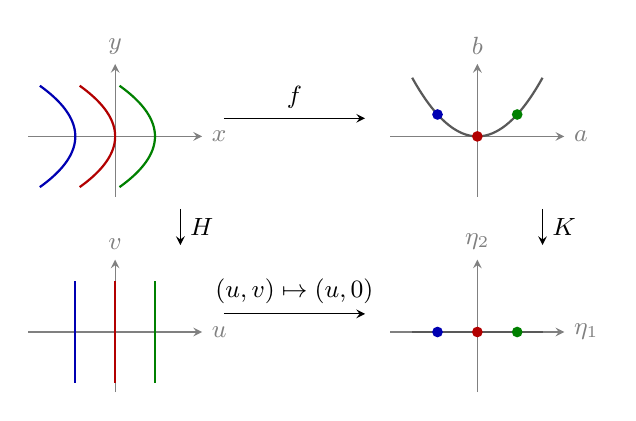
\begin{tikzpicture}[>=stealth,font=\small,scale=.92]
	\begin{scope}[yshift=2.7cm]
		\draw[->,gray] (-1.2,0)--(1.2,0) node[right] {\(x\)};
		\draw[->,gray] (0,-.83)--(0,1) node[above] {\(y\)};
		\foreach \level/\linecolour in {-.55/blue!70!black,0/red!70!black,.55/green!50!black}{
			\draw[thick,\linecolour,domain=-.7:.7,samples=40,variable=\t] plot ({\level-\t*\t},\t);
		}
	\end{scope}
	\begin{scope}[xshift=5cm,yshift=2.7cm]
		\draw[->,gray] (-1.2,0)--(1.2,0) node[right] {\(a\)};
		\draw[->,gray] (0,-.83)--(0,1) node[above] {\(b\)};
		\draw[thick,gray!70!black,domain=-.9:.9,samples=40] plot (\x,{\x*\x});
		\foreach \level/\linecolour in {-.55/blue!70!black,0/red!70!black,.55/green!50!black}{
			\fill[\linecolour] (\level,{\level*\level}) circle (2.1pt);
		}
	\end{scope}
	\draw[->] (1.5,2.95)--(3.45,2.95) node[midway,above] {\(f\)};
	\draw[->] (.9,1.7)--(.9,1.2) node[midway,right] {\(H\)};
	\draw[->] (5.9,1.7)--(5.9,1.2) node[midway,right] {\(K\)};
	\begin{scope}
		\draw[->,gray] (-1.2,0)--(1.2,0) node[right] {\(u\)};
		\draw[->,gray] (0,-.83)--(0,1) node[above] {\(v\)};
		\foreach \level/\linecolour in {-.55/blue!70!black,0/red!70!black,.55/green!50!black}{
			\draw[thick,\linecolour] (\level,-.7)--(\level,.7);
		}
	\end{scope}
	\begin{scope}[xshift=5cm]
		\draw[->,gray] (-1.2,0)--(1.2,0) node[right] {\(\eta_1\)};
		\draw[->,gray] (0,-.83)--(0,1) node[above] {\(\eta_2\)};
		\draw[thick,gray!70!black] (-.9,0)--(.9,0);
		\foreach \level/\linecolour in {-.55/blue!70!black,0/red!70!black,.55/green!50!black}{
			\fill[\linecolour] (\level,0) circle (2.1pt);
		}
	\end{scope}
	\draw[->] (1.5,.25)--(3.45,.25) node[midway,above] {\((u,v)\mapsto(u,0)\)};
\end{tikzpicture}


	\caption[常秩坐标如何同时整理原像与像]{例中的映射 \(f(x,y)=(x+y^2,(x+y^2)^2)\)。上排是原坐标，下排是经 \(H(x,y)=(x+y^2,y)\) 与 \(K(a,b)=(a,b-a^2)\) 改换后的坐标。同色源曲线映到同色目标点；新坐标使各条原像成为竖直线段，使像成为水平直线。图只显示选取的坐标范围。}
	\label{g1:fig:constant-rank-coordinates}
\end{figure}

\begin{corollary}[流形上的常秩标准形]
	\label{g1:cor:manifold-constant-rank}
	设 \(F:M^m\to N^n\) 是无边界光滑流形间的光滑映射，取 \(p\in M\)，且 \(\operatorname{rank}\mathrm{d}F_q=r\) 在 \(p\) 的某个邻域内恒定。则存在 \(p\) 与 \(F(p)\) 附近的光滑坐标，分别以这两点为原点，使 \(F\) 的坐标表达为 \((u^1,\ldots,u^m)\mapsto(u^1,\ldots,u^r,0,\ldots,0)\)，其中末尾有 \(n-r\) 个零，即\eqref{g1:eq:constant-rank-normal-form}。这里不要求坐标变化保持原先给定的度量、长度或角度。
\end{corollary}
\begin{proof}
	先选任意两张坐标图。由\cref{g1:def:manifold-differential,g1:prop:differential-chain-rule}，坐标表达的导数在两侧与坐标微分的可逆线性映射复合，所以它的秩恰为 \(\mathrm{d}F\) 的秩。Euclid 常秩定理给出源、目标坐标域中的进一步微分同胚；将它们与原坐标图复合，仍是光滑坐标图，就得到结论。构造只使用光滑可逆性，未施加任何度量限制。
\end{proof}

\subsection{秩不恒定时的反例}
\label{g1:subsec:1103:04}

常秩假设控制的是一个邻域，不是单点。单点的导数只记录一阶信息，不能独自判定附近原像的形状。不过微分矩阵的连续性确实提供一个有用的单侧结论。

\begin{proposition}
	\label{g1:prop:rank-lower-bound}
	对光滑映射 \(F:M^m\to N^n\)，若 \(\operatorname{rank}\mathrm{d}F_p\geq r\)，则在 \(p\) 的某个邻域中处处有 \(\operatorname{rank}\mathrm{d}F_q\geq r\)。特别地，若在 \(p\) 处秩达到最大可能值 \(\min(m,n)\)，则它在附近自动恒定。
\end{proposition}
\begin{proof}
	在坐标中，秩至少为 \(r>0\) 意味着某个 \(r\) 阶子式非零。该子式是导数矩阵元的多项式，随点连续，所以在足够小邻域中仍非零，秩遂仍至少为 \(r\)。当 \(r=0\) 时结论本身没有限制。最后秩始终不超过 \(\min(m,n)\)，因而达到这一上界时，邻域中的上下界相同。
\end{proof}

\begin{example}
	\label{g1:exm:cubic-rank-change}
	映射 \(f(t)=t^3\) 在原点的导数为零，在其余点的秩为 \(1\)。它仍是 \(\mathbb R\) 到自身的连续双射，逆函数为实立方根；但
	\[
		\frac{f^{-1}(h)-f^{-1}(0)}h=|h|^{-2/3}\longrightarrow\infty
		\qquad(h\to0),
	\]
	所以逆函数在零处不可微。导数可逆是局部光滑可逆的必要条件：若光滑逆存在，对两个复合恒等式求微分，便得到互逆的导数矩阵。它却不是连续可逆的必要条件，立方函数正好区分了这两件事。
\end{example}

在原点把 \(f\) 的秩记为零，并不能将立方函数在邻域中改成常值映射。任意可逆坐标变化都保持每一点的微分秩，而这个例子在任意原点邻域内都有秩为 \(1\) 的点。

\begin{example}
	\label{g1:exm:rank-changing-product}
	考虑 \(F(x,y)=(x,xy)\)，则
	\[
		\mathrm{D}F(x,y)=\begin{pmatrix}1&0\\y&x\end{pmatrix}.
	\]
	它在 \(x\ne0\) 时秩为 \(2\)，在整条 \(x=0\) 的直线上秩为 \(1\)。同值集合也发生明显变化：
	\[
		F^{-1}(a,b)=
		\begin{cases}
			\{(a,b/a)\},&a\ne0,\\
			\{(0,y):y\in\mathbb R\},&(a,b)=(0,0),\\
			\varnothing,&a=0,\ b\ne0.
		\end{cases}
	\]
	尤其在原点附近，整条短竖线被压到一点，旁边的点却各自局部可逆。若源邻域取为 \(|x|<\varepsilon,\ |y|<\delta\)，其像为
	\[
		\{(a,b):0<|a|<\varepsilon,\ |b|<\delta|a|\}\cup\{(0,0)\}.
	\]
	这个像在原点附近既不是开邻域，也不能由一段光滑坐标直线描述。常秩定理证明中的余分量在这里是 \(G(u,v)=uv\)，其 \(\mathrm{D}_vG=u\) 只在 \(u=0\) 上消失，不能因此删掉全部 \(v\) 依赖。
\end{example}

由此可见，若希望一个方程的解集或映射的原像具有稳定的局部维数，必须检查相应邻域中的正则条件。下一节将把满秩情形分别解释为浸入与淹没，并将这些坐标形式用于子流形；本节的结果只处理无边界邻域，半空间边界还需要相应的边界条件。

